% make sure not a repeat header!
\subsection{Getting started in EA}
\visHeader
\hypertarget{static:starting vis}{}

You can begin modeling Leitner's Box in two different ways. You can either continue in the same workspace as the Part I demo by opening the previous
\texttt{demo.eap} file in EA, initializating a new diagram and working within that space, or you can start this project with a clean slate by going to ``New
Metamodel Project,'' choosing to start a new visual project (without the demo specifications) (Fig.~\ref{fig:new_visModel}), and opening that empty
\texttt{.eap} file. This handbook has assumed you prefer the latter, which is reflected in the screenshots. If you use the previous file, please note that the
steps are exactly the same, but our package explorers may not match exactly. Keep a sharp eye out for footnotes which will explain the few differences.

\begin{figure}[htbp]
	\centering
  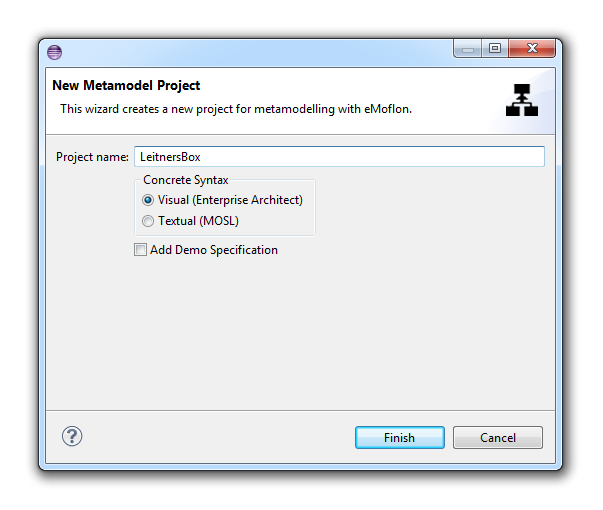
\includegraphics[width=0.9\textwidth]{eclipse_newMetamodelVisualPlain}
	\caption{Starting a new visual project}
	\label{fig:new_visModel}
\end{figure}

\newpage
\begin{itemize}
\item[$\blacktriangleright$] From EA, select your working set and press the ``Add a Package'' button (Fig.~\ref{fig:new_package}).

\begin{figure}[htbp]
	\centering
  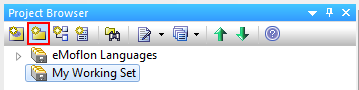
\includegraphics[width=0.5\textwidth]{ea_addPackage}
	\caption{Add a new package to \texttt{Demo}.}
	\label{fig:new_package}
	\vspace{0.5cm}
\end{figure}

\vspace{0.5cm}

\item[$\blacktriangleright$] In the dialogue that pops up (Fig.~\ref{fig:new_package_name}), enter 'Learning\-Box\-Language' as the name of the new package,
choose \texttt{Class View},  and click \texttt{OK}.

\begin{figure}[htbp]
	\centering
    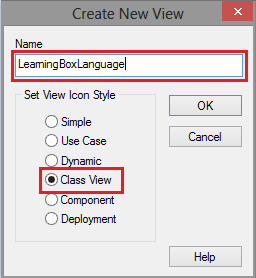
\includegraphics[width=0.33\textwidth]{ea_namePackage.png}
	\caption{Enter the name of the new package.}
	\label{fig:new_package_name}
\end{figure}
\FloatBarrier

\vspace{0.5cm}

\item[$\blacktriangleright$] Your \texttt{Project Browser} should now resemble Fig.~\ref{fig:new_package_completed}.

\begin{figure}[htbp]
	\centering
  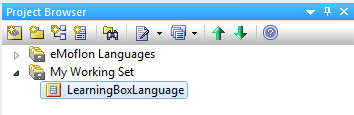
\includegraphics[width=0.5\textwidth]{ea_newPackage}
	\caption{State after creating the new package.}
	\label{fig:new_package_completed}
\end{figure}
\FloatBarrier

\clearpage
\item[$\blacktriangleright$] Now create a ``New Diagram'' (Fig.~\ref{fig:diagram}).

\begin{figure}[htbp]
	\centering
  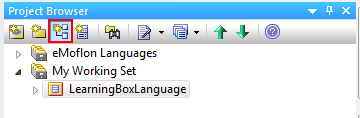
\includegraphics[width=0.5\textwidth]{ea_addDiagram}
	\caption{Add a diagram.}
	\label{fig:diagram}
\end{figure}
\FloatBarrier

\item[$\blacktriangleright$] In the dialogue that appears, (Fig.~\ref{fig:diagram_type}), choose \texttt{eMoflon Ecore Diagrams}, then press \texttt{OK}.

\begin{figure}[htbp]
	\centering
  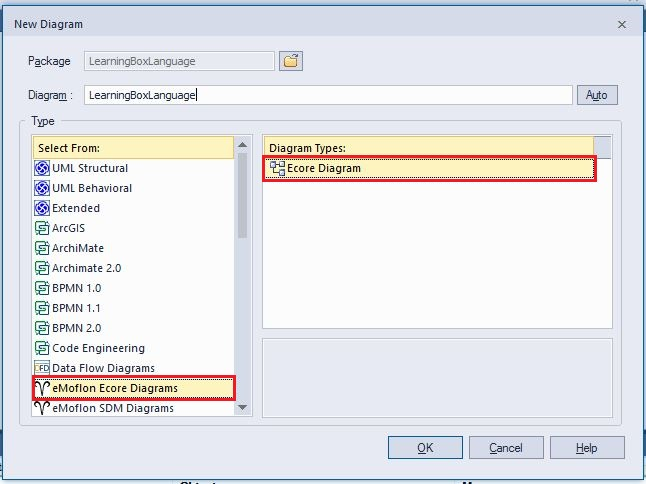
\includegraphics[width=0.8\textwidth]{ea_chooseDiagramType}
	\caption{Select the ecore diagram type}
	\label{fig:diagram_type}
\end{figure}
\FloatBarrier

 
\item[$\blacktriangleright$] After creating the new diagram, your  \texttt{Project Browser} should now resemble Fig.~\ref{fig:diagram_completed}.

\begin{figure}[htbp]
	\centering
  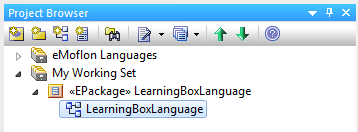
\includegraphics[width=0.5\textwidth]{ea_afterDiagramState}
	\caption{State after creating diagram}
	\label{fig:diagram_completed}
\end{figure}
\FloatBarrier

\item[$\blacktriangleright$] These are the basic steps for creating \emph{any} new metamodel. Your LearningBoxLanguage diagram will be the starting point, or
anchor, for each piece of this example program. All generated code is derived from this location. Your working set is able to hold several different projects at
once\footnote{which is the current case if you're continuing with the previous demo files.} some other comment here. Careful not to rehash.

\fancyfoot[R]{$\triangleright$ \hyperlink{static:classes vis}{Next}}
\end{itemize}
